\section{Methods}\label{sec:methods}
\begin{figure*}
    \centering
    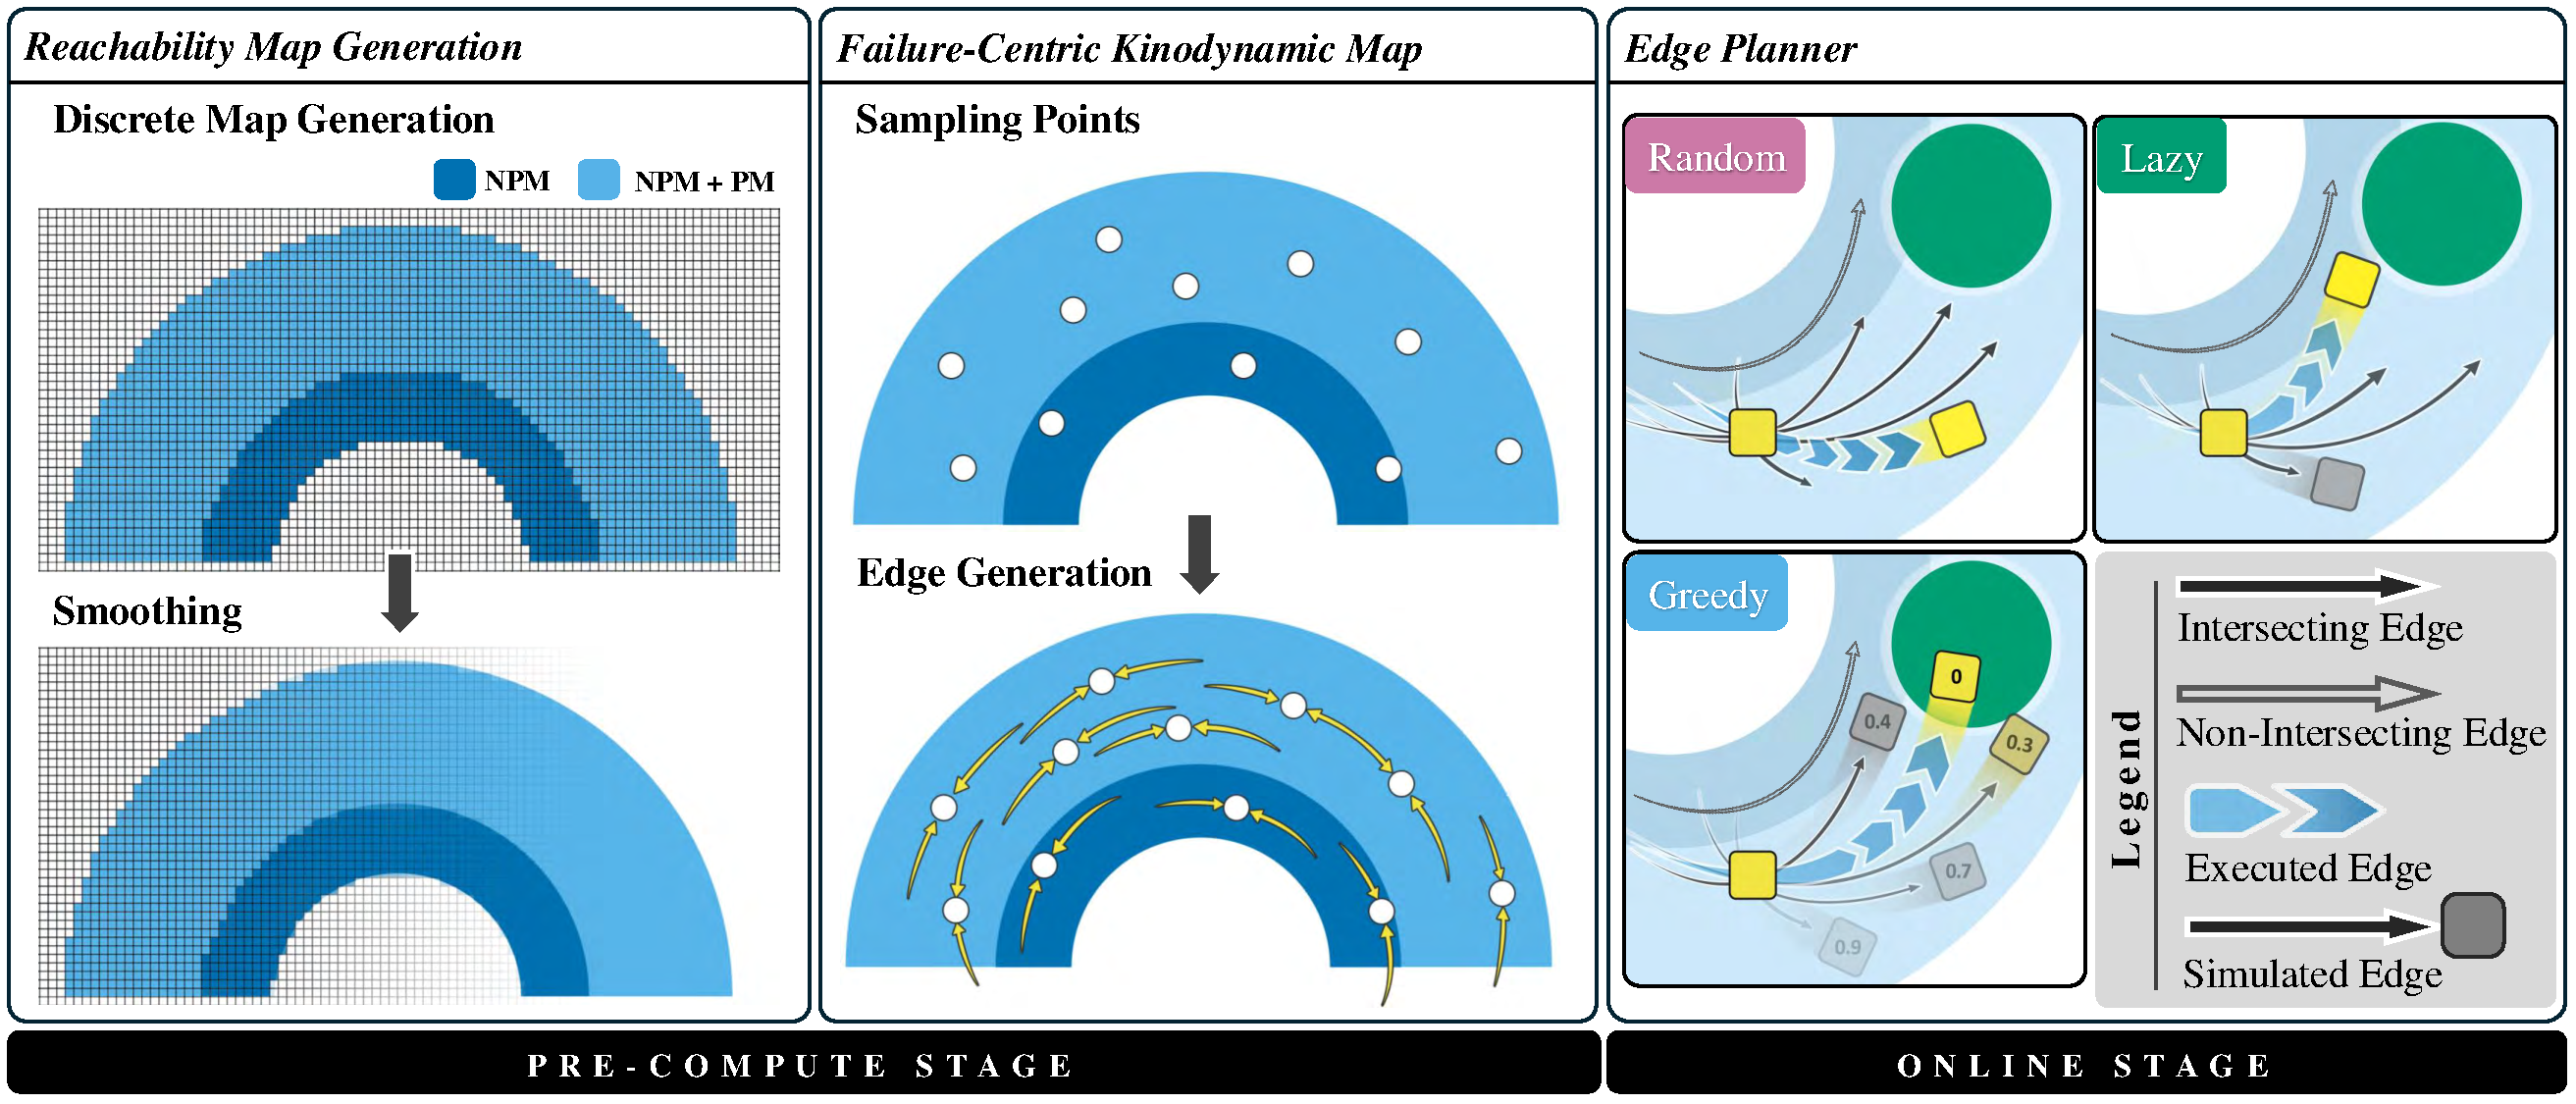
\includegraphics[width=\textwidth]{figures/Algorithm_Schematic-1-comp.pdf}
    \caption{An overview of the approach to expand manipulation capability in a robot experiencing LMJs. We generate a reachability map that captures the manipulation capability via \cref{algo:reachability} and smooth it with interpolation. We use this reachability map to determine the failure-centric kinodynamic map, via \cref{algo:generate-kinodynamic-manifold}, by sampling points in the reachable space and then saving dynamics rollouts (yellow arrows) as edges. To use this kinodynamic map, we developed an edge planner that can vary its use of sim-in-the-loop to determine which action the robot will take via the Random, Lazy, and Greedy Action Selection Mechanisms in \cref{algo:planner}. }
    \label{fig:methods}
\end{figure*}

To enable robotic arms to maintain operational utility in the face of locked multi-joint failures, our method diverges from traditional paradigms by employing non-prehensile manipulation, particularly poking actions, to extend the operational capabilities of robots after failure (\cref{sec:methods-npm}). By redefining motion primitives within the robot's new kinematic constraints, we explore an expanded operational space through a strategy that includes the pre-computation of reachable states (\cref{sec:methods-reachability}, \cref{fig:methods}, Left Column) and the formulation of kinodynamic edge bundles for feasible action planning (\cref{sec:methods-modeling}, \cref{fig:methods}, Center Column). We developed multiple approaches to selecting actions to understand the benefits of including a simulation in the planning and execution loop (\cref{sec:methods-planning}, \cref{fig:methods}, Right Column).



\subsection{Expanding Robot Capabilities through Non-Prehensile Manipulation}\label{sec:methods-npm}

%The prehensile perspective on robotic manipulation constrains existing approaches in enabling continuous robot operation in the presence of LMJs

Existing manipulation approaches cannot complete tasks in the presence of LMJs as they are restricted to exclusively prehensile actions. They regard grasping as a dependable method for engaging with the surroundings and consider the end-effector as the exclusive point of interaction between the robot and its environment.
Our approach challenges these notions by utilizing whole-body NPM to enhance the probability of task completion. 

We leverage the poking primitive in our work as a representative NPM ability to enable manipulation in the presence of LMJs since it significantly expands the set of reachable configurations and the number of degrees of freedom of the robot's operational space. Prior work has defined poking as a fundamental nonprehensile motion primitive
that is composed of two sequential phases: i) impact: a robot
end-effector applies an instantaneous force to an object at
rest, setting it in planar translational and rotational motion;
and, ii) free-sliding: the object slows down and comes to
a halt due to Coulomb friction between the object and its
support surface.  This primitive is not limited by robot
reach and leads to faster manipulation of objects in dense clutter, in the presence of occlusion, and in ungraspable configurations. \cite{pasricha2022pokerrt}

The challenge of identifying a viable sequence of NPM actions, such as poking, for a robot is exemplified by the high computational demands seen in algorithms like \textit{PokeRRT} \cite{pasricha2022pokerrt}. This process requires the simulation of numerous action sequences, many of which may prove infeasible for a specific robot failure mode. Therefore, this uniformly random exploration of the manifold of valid states and control parameters is inherently inefficient.
The complexity is further compounded when dealing with robots experiencing locked joint failures. In such scenarios, the search must look beyond only the space of control parameters for our chosen motion primitives and require these actions to be feasible within the altered kinematic landscape imposed by the failure. This intersection often leads to a zero-measure manifold, which is difficult to sample when following a uniformly random strategy.
To mitigate this issue, we propose a pre-computation approach, which maps the reach and capability post-LMJ and then finds a set of dynamic actions the robot can achieve, considering the limitations imposed by LMJs. This precomputed map of kinodynamically feasible actions serves as a guide, significantly reducing the computational overhead by providing a reference for what is achievable given the current failure mode.

\begin{algorithm}\footnotesize
    \caption{Generate Reach-Ability Map}\label{algo:reachability}

    \KwIn{$\mathcal{W}$, Workspace of the Robot; $\mathcal{X}$, set of joint constraints; $k$ replan attempts; $\epsilon$, perturbation radius}
    \KwOut{$\mathcal{W}^c$, the Failure-Constrained Workspace of the Robot}
    $iter = 0$ \\
    \For{$\mathbf{p} \in \mathcal{W}$}{
        \textsc{InteractionType} = ``PM" \\
        \textsc{InteractionArea} = ``End Effector" \\
        success $\longleftarrow$ inverseKinematics($\mathbf{p}$, $\mathcal{X}$, \textsc{InteractionType}, \textsc{InteractionArea}) \\
        \While{iter $< k$}{
            \If{iter $> 1$}{
                $\mathbf{\rho} \longleftarrow$ \textsc{SampleUniformEpsilonBall}($\epsilon$) \\
                $\mathbf{p}_{\rho} \longleftarrow \mathbf{p} + \mathbf{\rho}$ \\
                \If{iter $>k/2$}{
                \textsc{InteractionType}, \textsc{InteractionArea} $\longleftarrow$
                \textsc{ChangeInteraction}() }
                success $\longleftarrow$ \textsc{InverseKinematics}($\mathbf{p}_{\rho}$, $\mathcal{X}$, \textsc{InteractionType}, \textsc{InteractionArea})
            }            
            \If{success}{
                $\mathcal{W}^c \longleftarrow \mathcal{W}^c \cup \mathbf{p}$
                \break
            }
            $iter \longleftarrow iter + 1$ 
        }
    }
    \Return{$\mathcal{W}^c$}
\end{algorithm}


\subsection{Finding Reach and Manipulation Capability After Failure}\label{sec:methods-reachability}
When an LMJ occurs, the bounds of the robot's reachable workspace change in intractable, non-linear ways. We must understand the new reachable area and discover what manipulation capabilities the robot retains across this failure-constrained region to continue to complete tasks.

To do this, we developed a reachability and ability analysis system, or \textit{Reach-Ability} (\cref{algo:reachability}). The task space of the robot is divided into small areas approximately the size of the Franka Emika Panda end-effector tip, $2$ cm (\cref{fig:methods}, Left Column, Top). For each discretized area, we check to see if the robot can find an inverse kinematics solution for prehensile actions. To be considered a valid prehensile pose, the end-effector must be in a range of orientations that allow for grasping, nominally between normal to the workspace surface and parallel to the workspace surface. To counter the effects of the randomness of the inverse kinematics solver, if no solution is found initially, we uniformly sample a perturbation from an $\epsilon$-ball inscribed within the discretization cell and attempt solving again. 

If there is still no solution after half the replan attempts are calculated, \texttt{changeInteraction()} (\cref{algo:reachability}, L9) will release the orientation constraints of PM manipulation and switch to NPM abilities.%change the interaction type from PM to NPM
Under the NPM abilities, the inverse kinematics solver (\cref{algo:reachability}, L10) will: 1) cycle through pre-selected interaction points on the robot: hand, wrist, and forearm and 2) relax its orientation error bound so that the solution is only restricted in position. If no solutions are found, then that point is considered unreachable. The map is smoothed through interpolation once the whole task space is explored (\cref{fig:methods}, Left Column, Bottom).  
We leverage this mapping of the robot's statically reachable, failure-constrained workspace to build a representation of the robot's action manifold by utilizing the notion of edge bundles that parameterize the set of all feasible actions at the intersection of the post-failure-accessible manifold and the motion primitive manifold. 
% This still doesn’t allow for the execution of actions which leads us to a hierarchical representation - a notion of edge bundles that parameterize the set of all feasible actions at the intersection of the failure manifold and the motion primitive manifold. Brute force iteration.

% an understanding of the robot's failure-constrained workspace, we can now construct the kinodynamic map within those bounds.




\subsection{Construction of the Failure-Centric Kinodynamic Map}\label{sec:methods-modeling}

% \begin{itemize}
%     \item Introduce the notion of robot joint space manifold, $\mathcal{C}_q$
%     \item corresponding control space manifold $\mathcal{C}_u$
%     \item when a failure occurs, these manifolds are constrained, becoming $\mathcal{C}_q_c $ and$ \mathcal{C}_u_c$, respectively
%     \item $\mathcal{C}_q_c$ is constrained so much that finding valid plans via uniform random sampling and connecting them in $\mathcal{C}_u_c$ is unfeasible
%     \item so we use edge bundles to approximate $\mathcal{C}_q_c$ by forward propagating the robot's dynamics equation for a valid sampled control input in $\mathcal{C}_u_c$
%     \item each of these rollouts $r_q$ is saved in $\mathcal{E}$
% \end{itemize}

We can represent the set of all possible joint states and valid control inputs as the manifolds $\mathcal{C}$ and $\mathcal{U}$, respectively. We note the end-effector workspace of the robot as $\mathcal{W}$. When an LMJ occurs, these manifolds become degenerate, failure-constrained spaces. We note these constrained manifolds as $\mathcal{C}_c$, $\mathcal{U}_c$, and $\mathcal{W}_c$, respectively. 

The mapping between these spaces, $\mathcal{C} \mapsto \mathcal{C}_c$ and $\mathcal{U} \mapsto \mathcal{U}_c$, is nonlinear and dependent on the failure configuration of the robot. They also lose $n$ dimensions for $n$ locked joints. This degeneration means the failure-constrained manifolds have a significantly smaller volume than the unconstrained manifolds. As a result, the probability of finding a valid connecting plan between two uniformly, randomly sampled points in $\mathcal{C}_c$, with control inputs sampled from $\mathcal{U}_c$, approaches zero. \cite{kingston2018sampling}.

% Assuming a valid diagnosis of failure modes and the corresponding joint values for the locked joints, we follow a joint angle discretization approach on the remaining movable joints to map the robot's kinematically reachable space. 
Theoretically, an analytical solution to the inverse kinematics exists for any given point in $\mathcal{W}_c$. However, the multiple possible permutations of failures across the joints mean deriving the relevant equations or sampling valid configurations is untenable. As a result, we approximate $\mathcal{C}_c$ through a discretization-based approach.

We utilize the notion of edge bundles from \cite{shome2021asymptotically}. These edge bundles, $\mathcal{E}$, are a collection of Monte Carlo rollouts, or edges, $\mathbf{e}$ of the robot dynamical model with random control inputs, $\mathbf{\Dot{q}} \in \mathcal{U}_c$.
The nature of these edges, i.e., simulating a random control input from a random state for a random duration, ensures probabilistic completeness of the planning algorithm in \cref{sec:methods-planning} \cite{kleinbort2018probabilistic}. 
% (Note that claims on completeness may be inconclusive with respect to our planner since it uses the best-first input approach \cite{kleinbort2018probabilistic}.)
Following the procedure outlined in \cref{algo:generate-kinodynamic-manifold}, we use this Monte Carlo generation of edge bundles to produce a \textsl{failure-centric kinodynamic map} (\cref{fig:methods}, Center Column).
In practice, the set of all edges, $\mathcal{E}$, provides a discrete approximation to $\mathcal{C}_c$.

\begin{algorithm}\footnotesize

\caption{Generate Kinodynamic Manifold.}\label{algo:generate-kinodynamic-manifold}

\KwIn{$\mathcal{C}^c$, Constrained Configuration Space; $\mathcal{U}^c$, Constrained Control Space; $n$, number of samples; $\mathcal{W}^c$, failure-constrained workspace; $\Delta t$, the control timestep of the robot}
% ; $m_{min}$, the minimum acceptable manipulability measure
\KwOut{$\mathcal{E}$, a set of edges}

$\mathcal{E} \longleftarrow \emptyset$

\For{$i = 1 \ldots n$} {
    $\mathbf{e} \longleftarrow \emptyset$ \tcp{edge}
    $\xi_{EE} \longleftarrow$ \textsc{SamplePoint}($\mathcal{W}^c$) \tcp{XYZ Only}
    $\mathbf{q} \longleftarrow$ \textsc{PositionalInverseKinematics}($\xi_{EE}, \mathcal{C}^c$) \tcp{Orientation Unconstrained}
    $t \longleftarrow$ \textsc{SampleDuration}()\\
    $\mathbf{\dot{q}} \longleftarrow$ \textsc{SampleControlInput}($\mathcal{U}^c$) \\
    $valid \longleftarrow True$ \\
    \tcp{simulate}
    \While{\textsc{TimeRemaining}($t$)} {
        % $\dot{\mathbf{\dot{q}}} = \mathbf{0}$ \\ \tcp{const vel}
        $\ddot{\mathbf{q}} \longleftarrow J(\mathbf{q})^\dagger \times (\dot{\mathbf{\dot{q}}} - \dot{J}(\mathbf{q}))\mathbf{\dot{q}})$\\
        $\mathbf{\tau} \longleftarrow M(\mathbf{q})\ddot{\mathbf{q}} + C(\mathbf{q}, \mathbf{\dot{q}})\mathbf{\dot{q}} + g(\mathbf{q}) + f(\mathbf{\dot{q}})$\\
        $m \longleftarrow \sqrt{\det{J(\mathbf{q})J(\mathbf{q})^T}}$ \\
        \If{\textsc{LimitsViolated($\mathbf{q}$, $\ddot{\mathbf{q}}$, $\mathbf{\tau}$)} \textbf{or} \textsc{InCollision}($\mathbf{q}$)} 
        % \textbf{or} $m < m_{min}$
        { 
            $valid \longleftarrow False$\\
            \textbf{break}
        }
        $\mathbf{q}_{k+1} \longleftarrow \mathbf{q}_{k} + \mathbf{\dot{q}} \Delta t$ \\
        $\mathbf{e} \longleftarrow \mathbf{e} \cup \{\mathbf{q}_k, \mathbf{\dot{q}}\}$
    }
    \If{valid} {
            $\mathcal{E} \longleftarrow \mathcal{E} \cup \mathbf{e}$
    }

}
\Return{$\mathcal{E}$}

\end{algorithm}

A kinodynamic map is computed once offline for a given failure. Since NPM interactions are inherently stochastic, we explicitly only model the robot's dynamics in our edge bundle. These attributes allow reuse across many planning problems, making our motion planner multi-query. 




% \subsection{Planning for Failure Recovery}\label{sec:methods-planning}
\subsection{Motion Planning under LMJ Failure Conditions}\label{sec:methods-planning}

The \textsl{failure-constrained kinodynamic map} provides a set of actions for our planner to complete the manipulation task. It provides two main advantages in the context of failure-constrained motion planning: i) it removes the need for an inverse model such that no action sampling is required during the planning process, and ii) it caters to a multi-query planning framework to speed up planning times for the failure-case significantly. 
% \gm{add reason why multi-query is good}

\begin{algorithm}\footnotesize
\caption{Edge Planner.}\label{algo:planner}
\KwIn{$E$, The Environment State; $\mathcal{E}$, a set of edges; $m$, Action Selection Method Mode}
\KwOut{$\mathcal{A}$, an action for the robot to execute}

$\mathcal{T} \longleftarrow \emptyset$
% \textsc{TimeRemaining}() \textbf{or} 

\While{\textbf{not} \textsc{GoalReached($E$)}} {
    % node = \textsc{PickNode}()\\
    % \textsc{ResetEnvToState}(node)\\
    $\mathcal{E}_I \longleftarrow$
    \textsc{EdgesIntersectingObject}($\mathcal{E}$, $E$)\\
    \color{dusty_pink}
    \If{m=``Random"}{
        $e \longleftarrow \textsc{RandomUniformSelect}(\mathcal{E}_I)$\\
        $\mathcal{A} \longleftarrow e$ \\
        \Return{$\mathcal{A}$}
    }
    \color{dusty_green}
    \If{m=``Lazy"}{
        $E_{sim} \longleftarrow E $ \tcp{set sim env}
        \For{$\mathbf{e}$ in \textsc{SampleWithoutReplacement}($\mathcal{E}_I$)} {
            \textsc{SimulateRobotWithEdge($\mathbf{e}, E_{sim}$)} \\
            \If{\textsc{TargetMovedTowardsGoal}($E_{sim}$)}{
            $\mathcal{A} \longleftarrow \mathbf{e}$\\
            \textbf{break}
            }
        $E_{sim} \longleftarrow E$ \tcp{reset sim env}
        }
        \Return{$\mathcal{A}$}
    }
    \color{dusty_blue}
    \If{m=``Greedy"}{
        $\mathcal{A} \longleftarrow \emptyset$\\
    
        $\mathcal{E}_T \longleftarrow \emptyset$ \tcp{Edges Scored}
        $scores \longleftarrow \emptyset$ \\
        $\mathcal{E}_s \longleftarrow \textsc{UniformlySampleSubset}(\mathcal{E}_I)$ \\
        $E_{sim} \longleftarrow E $ \tcp{set sim env}
        \For{$\mathbf{e}$ in \textsc{SampleWithoutReplacement}($\mathcal{E}_s$)} {
            \textsc{SimulateRobotWithEdge($\mathbf{e}, E_{sim}$)} \\
            \If{\textsc{TargetMovedTowardsGoal}($E_{sim}$)}{
            $scores \longleftarrow scores \cup \textsc{ScoreExecution}(E_{sim}$)}
        $\mathcal{E}_T \longleftarrow \mathcal{E}_T \cup \mathbf{e} $ 
        
        
        $E_{sim} \longleftarrow E$ \tcp{reset sim env}
        }
         
        $\mathcal{A}\longleftarrow \textsc{SelectBestEdge}(\mathcal{E}_T, scores, m)$\\
        % $ \longleftarrow e_{best}$ \\
        % }
        \Return{$\mathcal{A}$}
    }
    % }
}

\end{algorithm}

% Keeping these advantages in mind, and based on the definition of the planning configuration space that supports multiple movable and fixed obstacles (\Cref{sec:methods}), we can formulate the multi--modal motion planning problem as follows:

% \begin{definition}[Multimodal Motion Planning Problem]
% Given the start configuration $x_{s} \in \mathcal{X}$ of an object at rest on a planar support surface, the \textsl{multimodal motion planning problem} finds a path $\mathcal{P} = ((x_{s}, x_{s+1}), (x_{s+1}, x_{s+2}), \dots, (x_{g-1}, x_g))$ in collision-free space $\mathcal{X}_{free} \subseteq \mathcal{X}$ to the desired goal object configuration $x_g \in \mathcal{X}$ under the influence of $p$ motion primitives, $MP_{1 \ldots p}$.
% \end{definition}

% This broad definition relies on several steps (\Cref{algo:multimodal-planner}) and we outline our design decisions next.


% \ap{explain each, and use; refer to algo}

% \subsubsection{Goal Region}\label{methods:goal-region}

% We focus on the task of relocating a single target object to the goal region. 
% Since multiple non--target objects in the scene can move under the influence of various motion primitives, our goal region is underspecified. Since the goal region is underspecific and computing the distance between every pair of movable objects is intractable in our problem definition involving multiple objects \ap{cite jenking's}, we calculate the distance from target object pose in the planning tree (\Cref{algo:multimodal-planner}, L2) when picking the nearest node to this sampled node. This incentivizes the planner to move the target object more than non--target objects.

% \subsubsection{Picking a Node}

% As is standard with most randomized kinodynamic planners \ap{cite}, we either sample a random node ($x_{rand} \in O$) or the goal node ($x_g$) if $rand(0, 1) < b_G$. Since the goal region is underspecific and computing the distance between every pair of movable objects is intractable in our problem setup involving multiple objects \ap{cite jenking's}, we calculate the distance from target object pose in the planning tree (\Cref{algo:multimodal-planner}, L2) when picking the nearest node to this sampled node. This influences the planner to move the target object more so than non--target objects and provides a solution to . Additionally, 

% \begin{algorithm}\footnotesize

\caption{Pick Actions.}\label{algo:pick-actions}

\KwIn{$n$, number of samples; $e$, edges; $o$, movable objects;\\$b_{RA}$, random action bias; $b_{IA}$, indirect action bias}
\KwOut{$\mathcal{A}$, chosen actions}

$\mathcal{I}, \mathcal{O} \longleftarrow$ \textsc{FindIntersectingEdges}($e$, $o$)\\

$objects \longleftarrow \emptyset$\\
$ee \longleftarrow \emptyset$\\
$\mathcal{I}_{target}, \mathcal{O}_{target} \longleftarrow$ \textsc{FindTarget}($e$, $o$)\\
\If{$rand() > b_{IA}$} {
    $ee \longleftarrow ee \cup I_{target}$
}
\Else {
    $ee \longleftarrow ee \cup (I \cap I_{target})$
}

$\mathcal{A} \longleftarrow \emptyset$ \\
$n_{rand} = b_{RA} * n$

\For{i = 1 \ldots n} {
    \For{j = 1 \ldots $n_{rand}$} {
        $\mathcal{A} \longleftarrow \mathcal{A} \; \cup$ \textsc{PickRandom}($e$)\\
    }
    $sorted\_e \longleftarrow$ \textsc{PriorityQueue}($e$)\\
    \For{j = 1 \ldots $n - n\_rand$} {
        $a \longleftarrow$ \textsc{POP}($sorted\_e$)\\
        \If{$a \notin \mathcal{A}$}{
            $\mathcal{A} \longleftarrow \mathcal{A} \cup a$
        }
    }
}

\Return{$\mathcal{A}$}

\end{algorithm}

% \begin{algorithm}\footnotesize

\caption{Random Action Selection}\label{algo:random-asm}
\color{dusty_pink}
\KwIn{$\mathcal{E}$, a set of edges; $E$ environment state}
%$\mathcal{C}^c$, Failure-Constrained Configuration Space;
\KwOut{$\mathcal{A}$, Chosen Action}

$e \longleftarrow \textsc{RandomUniformSelect}(\mathcal{E})$\\
$\mathcal{A} \longleftarrow e$ \\
\Return{$\mathcal{A}$}

\end{algorithm}
% \begin{algorithm}\footnotesize

\caption{Lazy Action Selection}\label{algo:lazy-asm}
\color{dusty_green}
\KwIn{$\mathcal{E}$, a set of edges; $E$ environment state}
\KwOut{$\mathcal{A}$, Chosen Action}
$E_{sim} \longleftarrow E $ \tcp{set sim env}\\ 
\For{$\mathbf{e}$ in \textsc{SampleWithoutReplacement}($\mathcal{E}_s$)} {
    \textsc{SimulateRobotWithEdge($\mathbf{e}, E_{sim}$)} \\
    \If{\textsc{TargetMovedTowardsGoal}($E_{sim}$)}{
    $\mathcal{A} \longleftarrow \mathbf{e}$\\
    \textbf{break}
    }
$E_{sim} \longleftarrow E$ \tcp{reset sim env}
}
\Return{$\mathcal{A}$}

\end{algorithm}
% \begin{algorithm}\footnotesize

\caption{Greedy Action Selection}\label{algo:greedy-asm}
\color{dusty_blue}
\KwIn{$\mathcal{E}$, a set of edges; $E$ environment state}
%$\mathcal{C}^c$, Failure-Constrained Configuration Space;
\KwOut{$\mathcal{A}$, Chosen Action}
$\mathcal{A} \longleftarrow \emptyset$\\
% \While{\textbf{not} \textsc{ObjectInGoalRegion}($E$)}{

$\mathcal{E}_T \longleftarrow \emptyset$ \tcp{Edges Scored}\\
$scores \longleftarrow \emptyset$ \\
$\mathcal{E}_s \longleftarrow \textsc{UniformlySampleSubset}(\mathcal{E})$ \\
$E_{sim} \longleftarrow E $ \tcp{set sim env}\\ 
\For{$\mathbf{e}$ in \textsc{SampleWithoutReplacement}($\mathcal{E}_s$)} {
    \textsc{SimulateRobotWithEdge($\mathbf{e}, E_{sim}$)} \\
    \If{\textsc{TargetMovedTowardsGoal}($E_{sim}$)}{
    $scores \longleftarrow scores \cup \textsc{ScoreExecution}(E_{sim}$)}\\
$\mathcal{E}_T \longleftarrow \mathcal{E}_T \cup \mathbf{e} $ \\


$E_{sim} \longleftarrow E$ \tcp{reset sim env}
}
 
$\mathcal{A}\longleftarrow \textsc{SelectBestEdge}(\mathcal{E}_T, scores, m)$\\
% $ \longleftarrow e_{best}$ \\
% }
\Return{$\mathcal{A}$}

\end{algorithm}

% \subsubsection{Picking an Action}

% Picking a valid action requires finding intersections between the situated kinodynamic manifolds for each primitive \ap{cite} and current environment configuration. This yields a subset of relevant objects and edges, weighted by primitive--specific utility values. In order to balance exploration and exploitation during the planning in this high--dimensional space as well as ensure progress towards goal, we introduce the indirect action $b_{IA}$ and random action biases $b_{RA}$, in addition to the goal bias $b_g$ that is typical in kinodynamic motion planning approaches \ap{cite}. Actions are ordered in a priority queue and greedily selected if $rand(0, 1) > b_{RA}$. Otherwise, a random action is chosen. Additionally, actions can either be chosen for the target object or non--target, movable objects. This balance is dictated by the indirect action bias $b_{IA}$. A higher values caters to actions on non--target objects which is useful in a cluttered scenario.

% \subsubsection{Simulating Object Dynamics}



% Our planning approach is designed to take maximal advantage of the motion primitives available to the robot. We next show an extensive ablative analysis of our planner and a comparison to a baseline kinodynamic planner. Task success is independent of the robot's start and end states.

Based on the approximations of the configuration and control manifolds ($\mathcal{C}_c$ and $\mathcal{U}_c$), our use of nonprehensile actions and environmental contact with the full embodiment of the robot arm enhances task success in the presence of LMJs.
Given a start configuration of the scene $x_0 \in E$, the motion planning for the failure recovery problem is to find a trajectory $\tau: [0, 1] \rightarrow E_{free} \cap \mathcal{W}_c$ such that $\tau(0) = x_0$ and $\tau(1) \in E_{goal}$ (\cref{fig:methods}, Right Column). Success is manipulating the target object from its starting pose to the goal region (\cref{algo:planner}).
% We specifically leverage the concept of multiple modalities across PM and NPM skills to accomplish manipulation tasks in the face of LMJ. For example, if the end-effector joints are locked and positioned in a way such that the robot cannot grasp, as shown in \cref{fig:panda_crippled}, we take advantage of poking to interact with the object. 

While the failure-constrained kinodynamic manifold captures the robot dynamics, interactions with scene objects are unmodeled because physical properties, especially friction for NPM interactions, behave stochastically in the real--world \cite{ALBERTINI2021104242}. However, physics engines provide approximately realistic predictions of rigid body dynamics. We use the Bullet physics simulation engine in the planning loop to get the resultant pose $x_{k+1}$ \cite{coumans2021}.  This allows us to capture an approximation of robot and object dynamics faster and safer than execution on a real robot. 
% Each action execution follows a validity check to ensure all objects remain within workspace bounds and no collisions occur between movable objects and fixed obstacles (\Cref{algo:multimodal-planner}, L8).

% Our planner interleaves planning and execution to compensate for discrepancies between simulation and real-world dynamics (\cref{algo:adaptr}).
To understand the benefits of utilizing a simulator in the planning loop, we study multiple Action Selection Mechanisms (ASMs):
\begin{itemize}
    \item \textbf{\color{dusty_pink}Random} (\cref{algo:planner}, L4-7): The Random ASM finds all the edges that intersect the object and picks one randomly.
    \item \textbf{\color{dusty_green}Lazy} (\cref{algo:planner}, L8-16): The Lazy ASM utilizes our sim-in-the-loop planner to find an edge that moves the target object toward the goal. Of all the edges that intersect the object, it picks the first action that moves the target towards the goal in the simulator.
    \item \textbf{\color{dusty_blue}Greedy} (\cref{algo:planner}, L17-30): The Greedy ASM will sample a subset of the edges that intersect the object and score them based on how close the target object is to the goal after simulating the selected actions. It will command the highest-scored edge for the real robot.
\end{itemize}

% With every action, the planning step follows the specified ASM to minimize the distance between the target object and the goal region (\cref{algo:adaptr}, L13). More specifically, the ASMs select, without replacement, from a set of edges approximating the failure-centric kinodynamic manifold and intersecting the target object (\cref{fig:edge_selection}) at every planning iteration (\cref{algo:adaptr}, L6).
% % , from $\mathcal{E}$, $\mathcal{F}$, 
% These edges are simulated in PyBullet \cite{coumans2021} on the current environmental scene to get resultant object poses (\cref{algo:adaptr}, L7). %The planner is described graphically in \cref{fig:timeline}.

% NPM actions compensate for the robot's limited reachable workspace by increasing the effective manipulable area.
% Additionally, in the presence of multiple joint failures, the end-effector reachable space may not intersect with the goal region. Using non-end-effector links, combined with NPM actions, increases the likelihood of task-relevant contact between the robot and the environment.
% We discuss the method for determining the reachability of the robot under failure and nominal conditions in the following section.



% Now that we have the edges, we call Algo. \ref{algo:adaptr} and pass the generated edges. In Line 1, 

% While the target object has not reached the goal region, 

% it will find edges that intersect with the target object by calling Algo. \ref{algo:edges-score-inters}. In Algo. \ref{algo:edges-score-inters} it iterates over all the edges. In Line 3, the robot performs the edge in simulation by following the joint angle velocities encoded in the edge starting from the edge initial joint angles. It does this by using PyBullet \cite{coumans2021}. If the object position has changed (Algo. \ref{algo:edges-score-inters}, L4) 

% it will set the edge score.
% \ap{uninvert edge score in algo, do argmin}

% The closer the edge moves the object toward the goal, the higher the score of that specific edge (Algo. \ref{algo:edges-score-inters}, L 6). The reason we use PyBullet to check for intersections is that the robot can intersect with the object with any part of its body not just the end effector. Now that we have set the score of all intersecting edges, we select the edge with the highest score in Line 3 in Algo. \ref{algo:adaptr} and execute the edge in the real world. We will continue looping through until the target object reaches the goal region. 






